% !TeX TS-program = txs:///duck
\documentclass{standalone}
\usepackage{tikzducks}

\definecolor{bodya}{RGB}{147,112,219}
\definecolor{haira}{RGB}{244,164,96}
\definecolor{backa}{RGB}{255,69,0}
\definecolor{glasa}{RGB}{0,255,127} 

\definecolor{bodyb}{RGB}{176,224,230}
\definecolor{hairb}{RGB}{255,215,9}
\definecolor{backb}{RGB}{249,207,207}
\definecolor{glasb}{RGB}{255,0,0} 

\definecolor{bodyc}{RGB}{237,212,37}
\definecolor{hairc}{RGB}{255,140,0}
\definecolor{backc}{RGB}{30,144,255}
\definecolor{glasc}{RGB}{255,0,255} 

\definecolor{bodyd}{RGB}{0,100,0}
\definecolor{haird}{RGB}{255,0,0}
\definecolor{backd}{RGB}{148,244,0}
\definecolor{glasd}{RGB}{175,238,238} 

\begin{document}

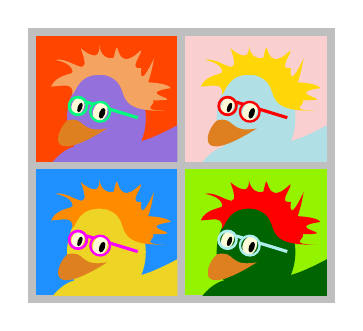
\begin{tikzpicture}

\fill[lightgray] (-0.1,-0.85) rectangle (3.8,2.65);

\begin{scope}
  \clip (0,0.95) rectangle (1.8,2.55);
  \fill[backa] (0,0.95) rectangle (1.8,2.55);

	\duck[
		body=bodya,
		crazyhair=haira,
		glasses=glasa
  ]
\end{scope}
  
\begin{scope}[xshift=1.9cm]
  \clip (0,0.95) rectangle (1.8,2.55);
  \fill[backb] (0,0.95) rectangle (1.8,2.55);

	\duck[
		body=bodyb,
		crazyhair=hairb,
		glasses=glasb
  ]
\end{scope}  

\begin{scope}[yshift=-1.7cm]
  \clip (0,0.95) rectangle (1.8,2.55);
  \fill[backc] (0,0.95) rectangle (1.8,2.55);

	\duck[
		body=bodyc,
		crazyhair=hairc,
		glasses=glasc
  ]
\end{scope}  

\begin{scope}[xshift=1.9cm,yshift=-1.7cm]
  \clip (0,0.95) rectangle (1.8,2.55);
  \fill[backd] (0,0.95) rectangle (1.8,2.55);

	\duck[
		body=bodyd,
		crazyhair=haird,
		glasses=glasd
  ]
\end{scope}  
  
\end{tikzpicture}	
	
\end{document}